\chapter{All Simulation Results}
\label{AppendixA}

This appendix documents the evolution of the CMOS inverter-based amplifier design through multiple versions. Each version addresses specific design challenges and improvements, validated through extensive simulations. Detailed results and schematics for each version are provided to illustrate the design iterations and their impact on performance.

\section{Version 1}

The first version of the design was based on the calculation of the transfer function using the DPSFG (Driving Point Signal Flow Graph) technique (see \textcite{Schmid_Huber_2018}). 
More details about this calculation can be found in the inv$\_$parameters.ipynb file on the GitHub repository \cite{miguelcorrea0107_2024}. 
This version had to be revised to incorporate active resistors due to size constraints.
\\
Figure \ref{fig:v1_schematic} shows the schematic of Version 1. 
The simulation results for this version are summarized in Table \ref{tab:v1_sim_results}.
\begin{figure}[ht!]
    \centering
    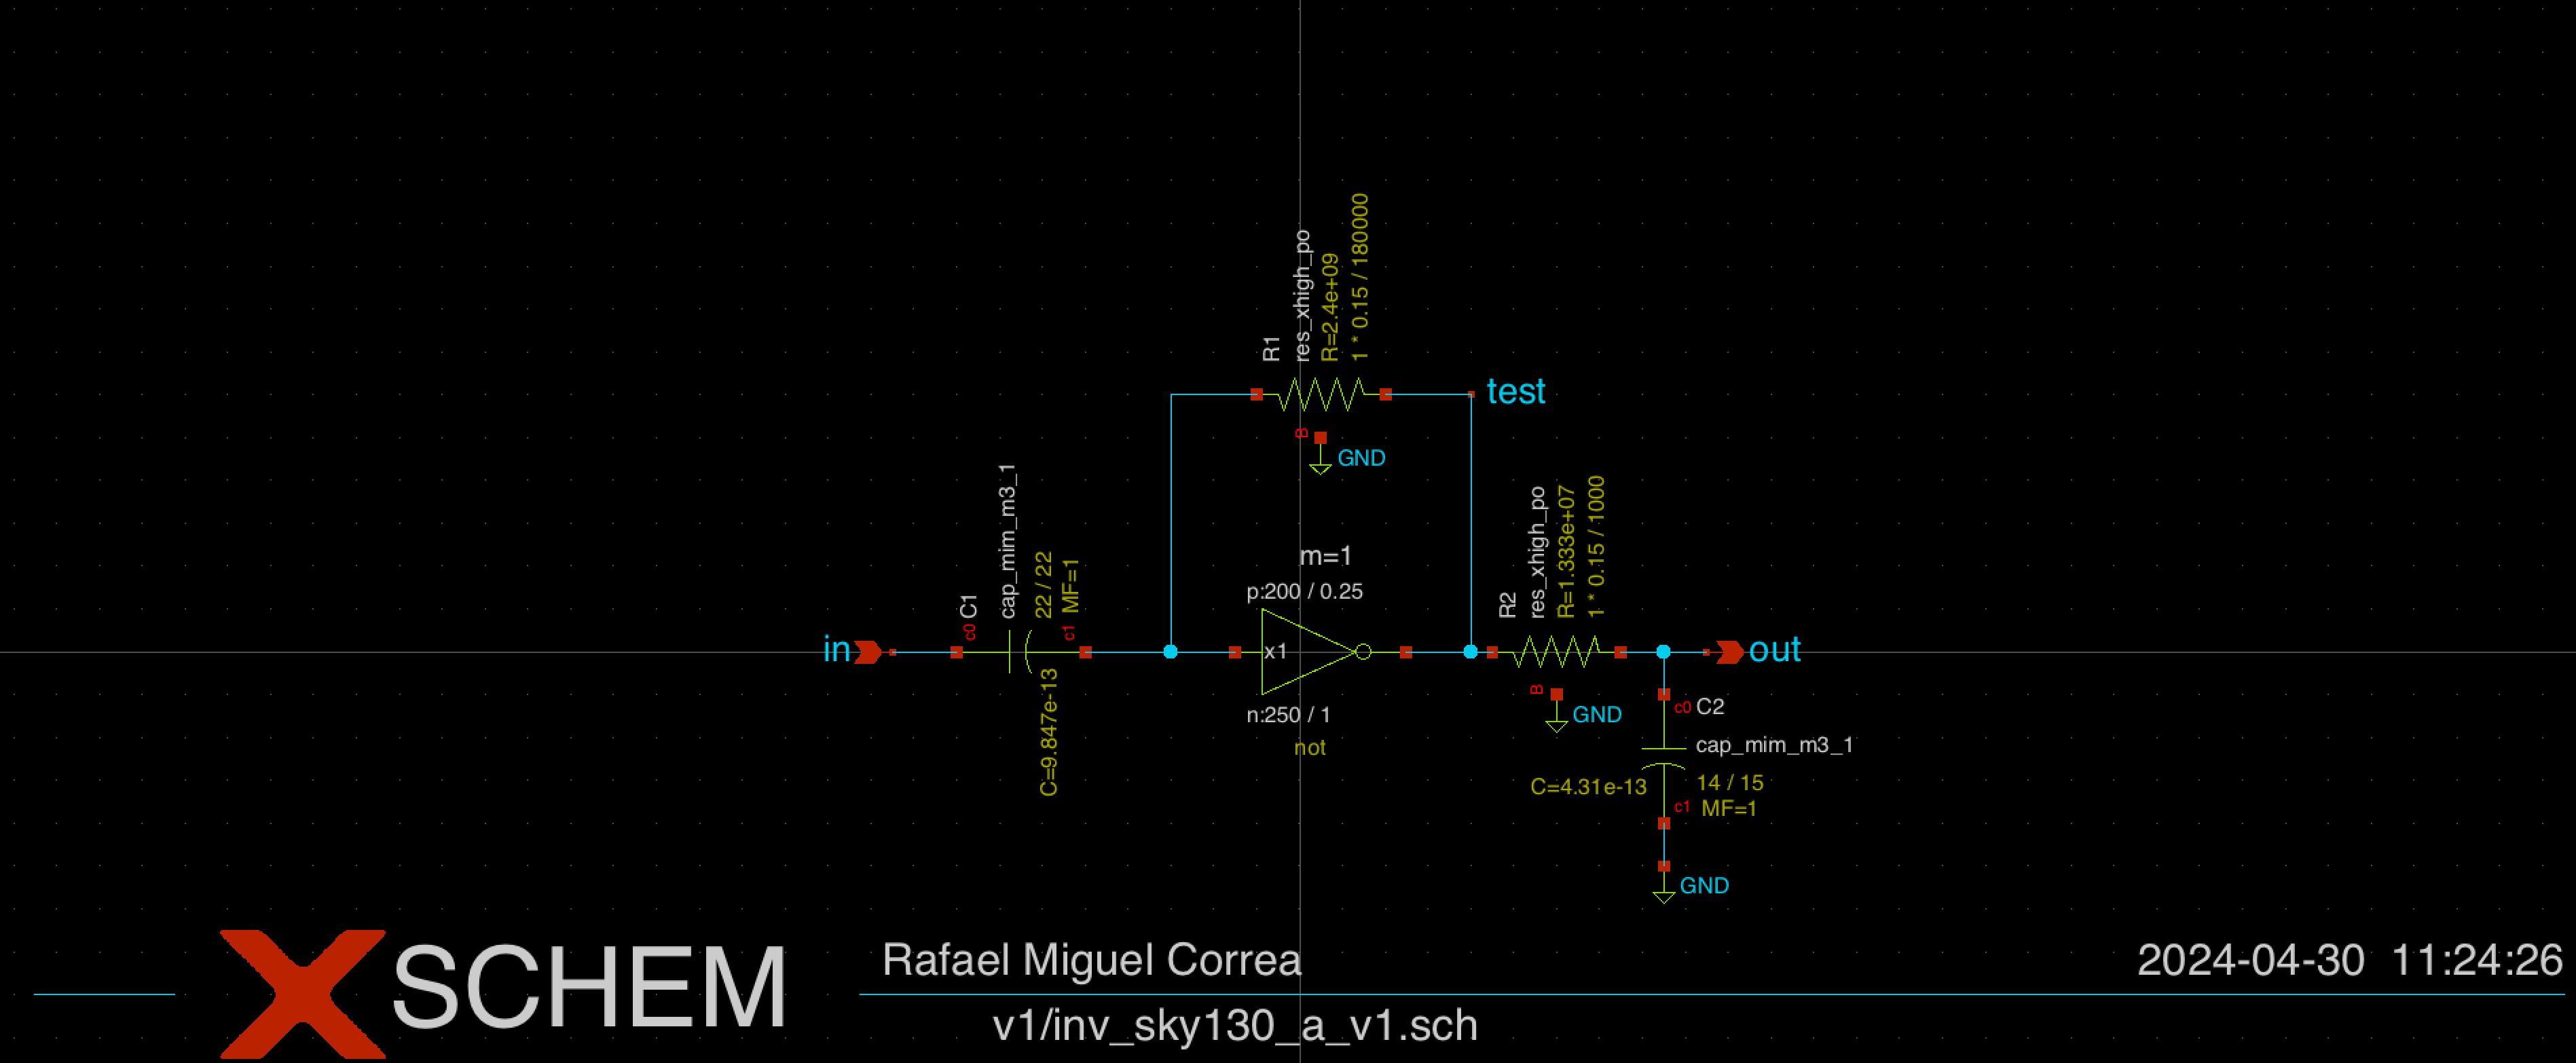
\includegraphics[width=\textwidth]{Figures/v1_schematic.png}
    \caption{Schematic of Version 1 of the CMOS inverter-based amplifier design.}
    \label{fig:v1_schematic}
\end{figure}

\begin{landscape}
\begin{table}[!ht]
    \centering
    \begin{adjustbox}{max width=\linewidth}
    \begin{tabular}{|c|c|c|c|c|c|c|c|c|c|c|c|c|c|c|}
        \hline
        \textbf{Vdd} & 1.5 & 1.25 & 1.125 & 1.125 & 1.125 & 1.125 & 1.125 & 1.125 & 1.125 & 1.125 & 1.125 & 1.125 & 1.125 & 1.125 \\ \hline
         \textbf{Wn} & 20.0 & 40.0 & 50.0 & 50.0 & 250.0 & 250.0 & 250.0 & 250.0 & 250.0 & 250.0 & 250.0 & 250.0 & 250.0 & 250.0 \\ \hline
            \textbf{Ln} & 0.15 & 0.15 & 0.15 & 0.15 & 1.0 & 1.0 & 1.0 & 1.0 & 1.0 & 1.0 & 1.0 & 1.0 & 1.0 & 1.0 \\ \hline
            \textbf{Wp} & 40.0 & 80.0 & 100.0 & 100.0 & 200.0 & 200.0 & 200.0 & 200.0 & 200.0 & 200.0 & 200.0 & 200.0 & 200.0 & 200.0 \\ \hline
            \textbf{Lp} & 0.15 & 0.15 & 0.15 & 0.15 & 0.25 & 0.25 & 0.25 & 0.25 & 0.25 & 0.25 & 0.25 & 0.25 & 0.25 & 0.25 \\ \hline
            \textbf{Wr1} & 1.0 & 1.0 & 1.0 & 1.0 & 1.0 & 1.0 & 0.15 & 0.15 & 0.15 & 0.15 & 0.15 & 0.15 & 0.15 & 0.15 \\ \hline
            \textbf{Lr1} & 30.0 & 50.0 & 90.0 & 90.0 & 90.0 & 90.0 & 100.0 & 100.0 & 250.0 & 300.0 & 300.0 & 25000.0 & 200000.0 & 200000.0 \\ \hline
            \textbf{R1 (in KOhms)} & 60.0 & 100.0 & 180.0 & 180.0 & 180.0 & 180.0 & 1333.333 & 1333.333 & 3333.333 & 4000.0 & 4000.0 & 333333.3 & 2666667.0 & 2666667.0 \\ \hline
            \textbf{Wr2} & 1.0 & 1.0 & 1.0 & 1.0 & 1.0 & 1.0 & 0.15 & 0.15 & 0.3 & 0.4 & 0.15 & 0.15 & 0.15 & 0.15 \\ \hline
            \textbf{Lr2} & 50.0 & 50.0 & 50.0 & 50.0 & 50.0 & 50.0 & 1.0 & 10.0 & 1.0 & 20.0 & 10.0 & 500.0 & 1000.0 & 1000.0 \\ \hline
            \textbf{R2 (in KOhms)} & 100.0 & 100.0 & 100.0 & 100.0 & 100.0 & 100.0 & 13.33333 & 133.33329999999998 & 6.666667 & 100.0 & 133.33329999999998 & 6666.667 & 13333.33 & 13333.33 \\ \hline
            \textbf{Wc1} & 0.0 & 0.0 & 0.0 & 0.0 & 0.0 & 0.0 & 22.0 & 22.0 & 100.0 & 100.0 & 170.0 & 42.0 & 13.0 & 22.0 \\ \hline
            \textbf{Lc1} & 0.0 & 0.0 & 0.0 & 0.0 & 0.0 & 0.0 & 22.0 & 22.0 & 100.0 & 100.0 & 170.0 & 42.0 & 13.0 & 22.0 \\ \hline
            \textbf{MFc1} & 0.0 & 0.0 & 0.0 & 0.0 & 0.0 & 0.0 & 1.0 & 1.0 & 1.0 & 1.0 & 1.0 & 1.0 & 1.0 & 1.0 \\ \hline
            \textbf{C1 (in PF)} & 0.0 & 0.0 & 0.0 & 0.0 & 0.0 & 0.0 & 0.98472 & 0.98472 & 20.076 & 20.076 & 57.929199999999994 & 3.55992 & 0.34787999999999997 & 0.98472 \\ \hline
            \textbf{Wc2} & 15.0 & 15.0 & 14.0 & 70.0 & 70.0 & 55.0 & 50.0 & 50.0 & 100.0 & 170.0 & 250.0 & 47.0 & 14.0 & 14.0 \\ \hline
            \textbf{Lc2} & 15.0 & 15.0 & 13.0 & 60.0 & 60.0 & 55.0 & 50.0 & 50.0 & 100.0 & 170.0 & 250.0 & 48.0 & 15.0 & 15.0 \\ \hline
            \textbf{MFc2} & 6.0 & 6.0 & 6.0 & 6.0 & 6.0 & 5.0 & 1.0 & 1.0 & 1.0 & 1.0 & 1.0 & 1.0 & 1.0 & 1.0 \\ \hline
            \textbf{C2 (in PF)} & 2.768 & 2.768 & 2.246 & 50.699999999999996 & 50.6964 & 30.459000000000003 & 5.038 & 5.038 & 20.076 & 57.929199999999994 & 125.19000000000001 & 4.5481 & 0.43102 & 0.43102 \\ \hline
            \textbf{Vdc (in MV)} & 705.2 & 590.0999999999999 & 538.0 & 538.0 & 448.66 & 448.66 & 448.66 & 448.66 & 448.66 & 448.66 & 448.66 & 448.66 & 448.66 & 448.66 \\ \hline
            \textbf{Gain (in DB)} & 20.51506 & 20.22268 & 20.17452 & 20.17452 & 23.82489 & 23.82489 & 14.74058 & 3.778642 & 31.82523 & 24.36886 & 20.45644 & 22.77707 & 7.736271 & 16.13267 \\ \hline
            \textbf{Lower Cut-Off Frequency (in Hz)} & 0.0 & 0.0 & 0.0 & 0.0 & 0.0 & 0.0 & 158489.3 & 62661.39 & 19364.22 & 8147.043 & 2213.095 & 606.7363 & 162.5549 & 150.6607 \\ \hline
            \textbf{Upper Cut-Off Frequency (in KHz)} & 525.0492 & 489.2721 & 519.937 & 23.02707 & 12.94196 & 21.51295 & 403645.4 & 411149.7 & 41399.97 & 22233.1 & 10000.0 & 3706.807 & 10715.19 & 10665.96 \\ \hline
            \textbf{Noise In (uV)} & 15.43656 & 9.761662 & 8.460034 & 8.460322 & 2.832653 & 2.832481 & 136.7781 & 136.7782 & 3.920957 & 3.632231 & 2.871612 & 3.833044 & 27.8819 & 11.58093 \\ \hline
            \textbf{Power (in UW)} & 161.3881 & 30.48936 & 9.831864 & 9.831872 & 2.794655 & 2.794644 & 2.794441 & 2.794441 & 2.794434 & 2.794422 & 2.794327 & 2.794165 & 2.794416 & 2.794374 \\ \hline
    \end{tabular}
    \end{adjustbox}
    \caption{Simulation results for Version 1 of the CMOS inverter-based amplifier design.}
    \label{tab:v1_sim_results}
\end{table}
\end{landscape}

\section{Version 2}
This version incorporated active resistors but encountered issues due to incorrect biasing of the resistors.
\\
Figure \ref{fig:v2_schematic} shows the schematic of Version 2. 
The simulation results for this version are summarized in Table \ref{tab:v2_sim_results}.
\begin{figure}[ht!]
    \centering
    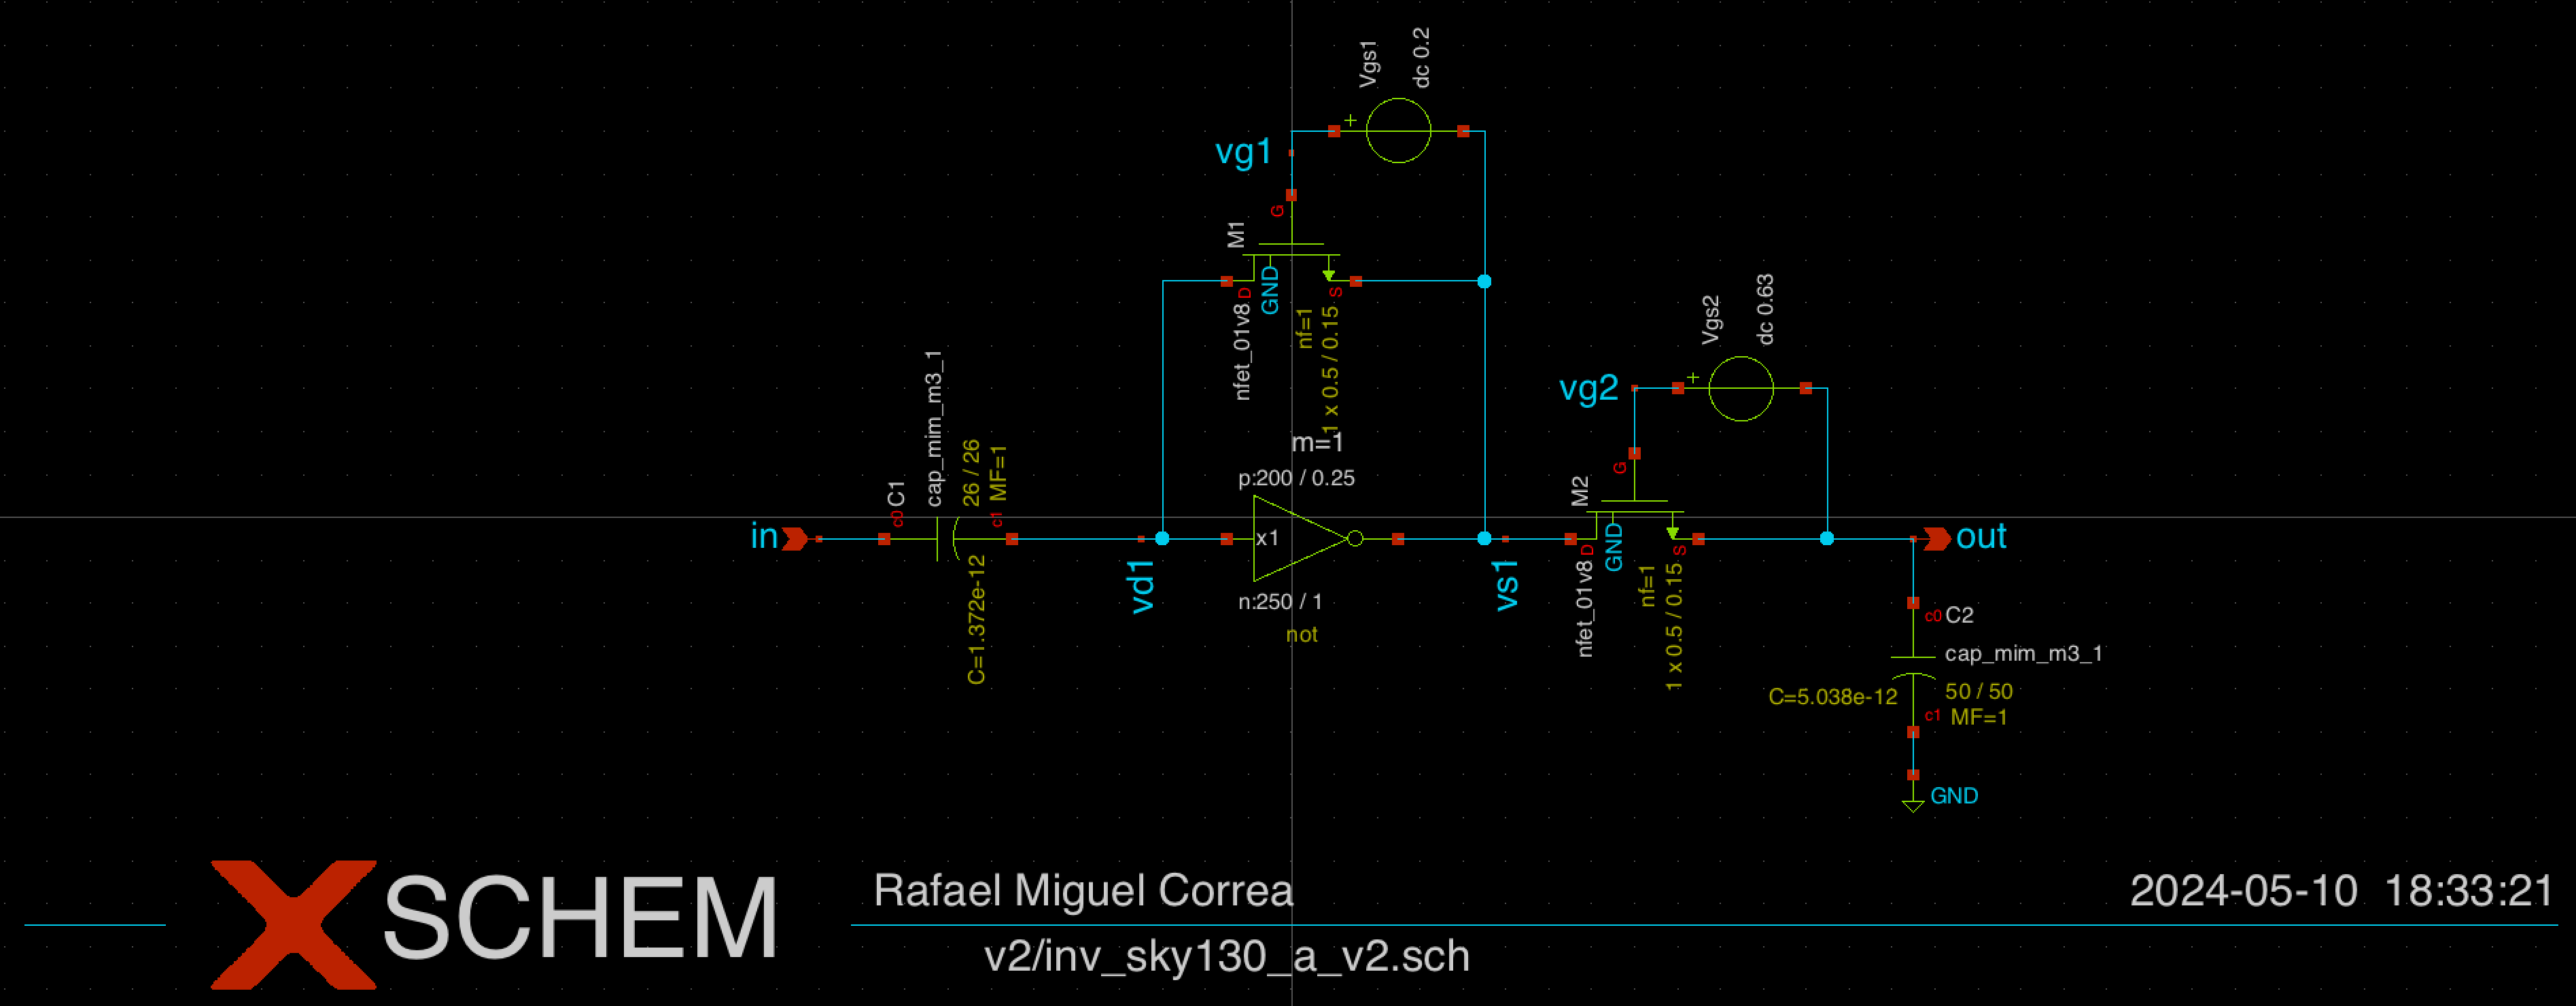
\includegraphics[width=\textwidth]{Figures/v2_schematic.png}
    \caption{Schematic of Version 2 of the CMOS inverter-based amplifier design.}
    \label{fig:v2_schematic}
\end{figure}

%\begin{landscape}
\begin{table}[!ht]
    \centering
    \begin{adjustbox}{max width=\linewidth}
    \begin{tabular}{|c|c|c|c|c|c|}
    \hline
        \textbf{Vdd} & 1.125 & 1.125 & 1.125 & 1.125 & 1.125 \\ \hline
        \textbf{Wn} & 250.0 & 250.0 & 250.0 & 250.0 & 250.0 \\ \hline
        \textbf{Ln} & 1.0 & 1.0 & 1.0 & 1.0 & 1.0 \\ \hline
        \textbf{Wp} & 200.0 & 200.0 & 200.0 & 200.0 & 200.0 \\ \hline
        \textbf{Lp} & 0.25 & 0.25 & 0.25 & 0.25 & 0.25 \\ \hline
        \textbf{R1\_Wn} & 0.5 & 0.5 & 0.5 & 0.5 & 0.5 \\ \hline
        \textbf{R1\_Ln} & 0.15 & 0.15 & 0.15 & 0.15 & 0.15 \\ \hline
        \textbf{R1\_Vgs} & 0.35 & 0.3 & 0.26 & 0.26 & 0.2 \\ \hline
        \textbf{R2\_Wn} & 0.5 & 0.5 & 0.5 & 0.5 & 0.5 \\ \hline
        \textbf{R2\_Ln} & 0.15 & 0.15 & 0.15 & 0.15 & 0.15 \\ \hline
        \textbf{R2\_Vgs} & 0.5 & 0.55 & 0.6 & 0.6 & 0.63 \\ \hline
        \textbf{Wc1} & 22.0 & 22.0 & 26.0 & 26.0 & 26.0 \\ \hline
        \textbf{Lc1} & 22.0 & 22.0 & 26.0 & 26.0 & 26.0 \\ \hline
        \textbf{MFc1} & 1.0 & 1.0 & 1.0 & 1.0 & 1.0 \\ \hline
        \textbf{C1 (in pF)} & 0.98472 & 0.98472 & 1.37176 & 1.37176 & 1.37176 \\ \hline
        \textbf{Wc2} & 14.0 & 14.0 & 30.0 & 35.0 & 50.0 \\ \hline
        \textbf{Lc2} & 15.0 & 15.0 & 30.0 & 35.0 & 50.0 \\ \hline
        \textbf{MFc2} & 1.0 & 1.0 & 1.0 & 1.0 & 1.0 \\ \hline
        \textbf{C2 (in pF)} & 0.43102 & 0.43102 & 1.8228 & 2.4766000000000004 & 5.038 \\ \hline
        \textbf{Vdc (in mV)} & 450.0 & 450.0 & 450.0 & 450.0 & 448.66 \\ \hline
        \textbf{gain (in dB)} & 18.08885 & 18.51345 & 20.90514 & 20.89836 & 20.8709 \\ \hline
        \textbf{lower cut-off frequency (in Hz)} & 220.2926 & 72.4436 & 33.72873 & 33.72873 & 20.6063 \\ \hline
        \textbf{upper cut-off frequency (in Hz)} & 4886.524 & 17701.09 & 15135.61 & 11168.63 & 10069.32 \\ \hline
        \textbf{noise in (uV)} & 14.97764 & 8.773817 & 5.699407 & 5.699722 & 5.444804 \\ \hline
        \textbf{power (in uW)} & 2.792742 & 2.787491 & 2.777074 & 2.777075 & 2.747301 \\ \hline
    \end{tabular}
    \end{adjustbox}
    \caption{Simulation results for Version 2 of the CMOS inverter-based amplifier design.}
    \label{tab:v2_sim_results}
\end{table}
%\end{landscape}

\section{Version 3}
The third version fixed the biasing of the active resistors, addressing the issues found in the previous version.
\\
Figure \ref{fig:v3_schematic} shows the schematic of Version 3. 
The simulation results for this version are summarized in Table \ref{tab:v3_sim_results}.
\begin{figure}[ht!]
    \centering
    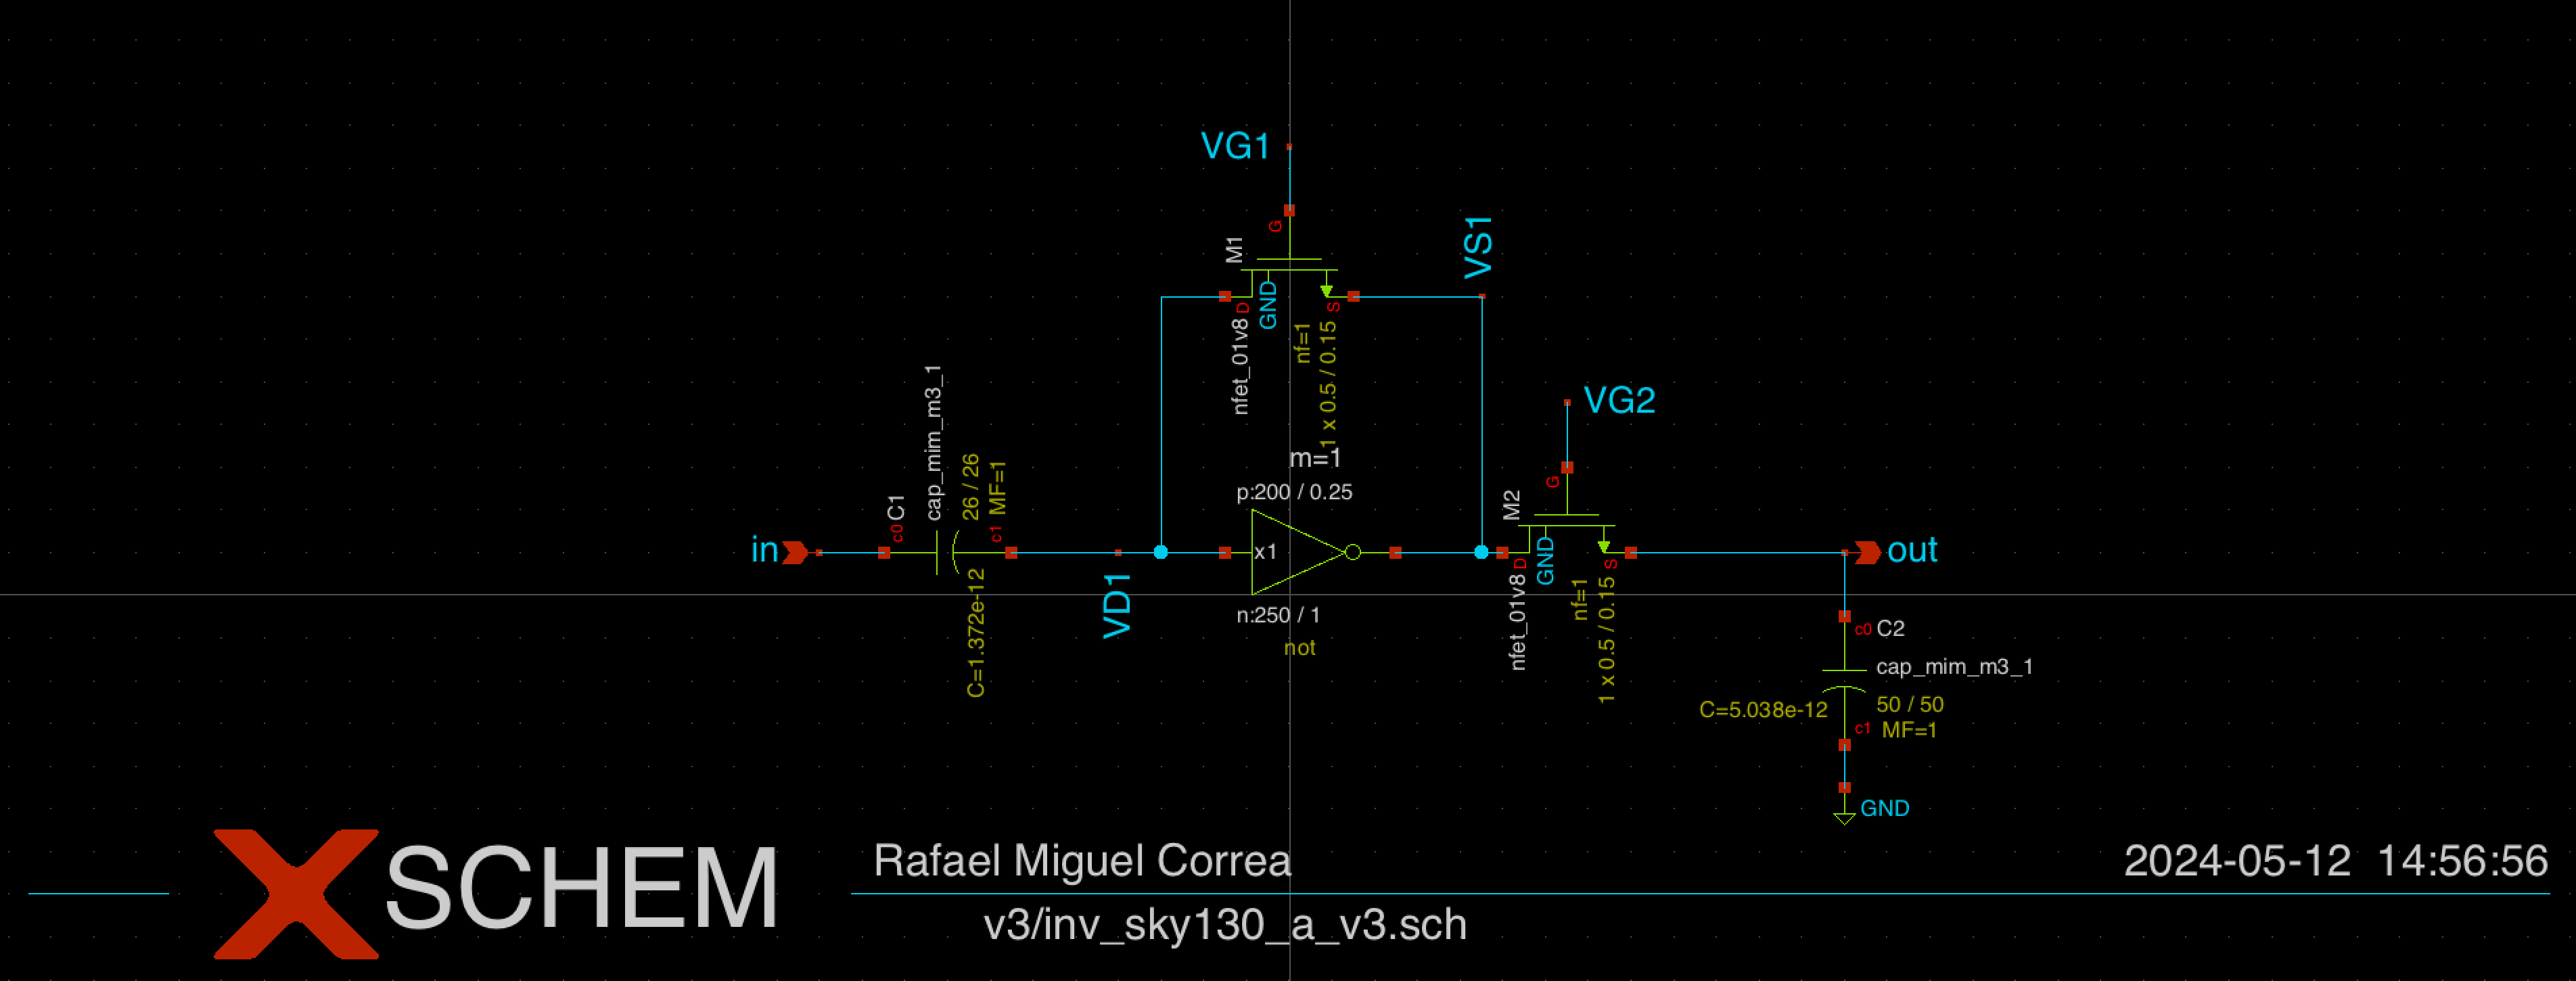
\includegraphics[width=\textwidth]{Figures/v3_schematic.png}
    \caption{Schematic of Version 3 of the CMOS inverter-based amplifier design.}
    \label{fig:v3_schematic}
\end{figure}

%\begin{landscape}
\begin{table}[!ht]
    \centering 
    \begin{adjustbox}{max width=\linewidth}
    \begin{tabular}{|c|c|c|c|c|}
    \hline
        \textbf{Vdd} & 1.125 & 1.125 & 1.125 & 1.125 \\ \hline
        \textbf{Wn} & 250.0 & 250.0 & 250.0 & 250.0 \\ \hline
        \textbf{Ln} & 1.0 & 1.0 & 1.0 & 1.0 \\ \hline
        \textbf{Wp} & 200.0 & 200.0 & 200.0 & 200.0 \\ \hline
        \textbf{Lp} & 0.25 & 0.25 & 0.25 & 0.25 \\ \hline
        \textbf{R1\_Wn} & 0.5 & 0.5 & 0.5 & 0.5 \\ \hline
        \textbf{R1\_Ln} & 0.15 & 0.15 & 0.15 & 0.15 \\ \hline
        \textbf{R1\_Vg} & 0.714 & 0.714 & 0.725 & 0.725 \\ \hline
        \textbf{R2\_Wn} & 0.5 & 0.5 & 0.5 & 0.5 \\ \hline
        \textbf{R2\_Ln} & 0.15 & 0.15 & 0.15 & 0.15 \\ \hline
        \textbf{R2\_Vg} & 1.14439 & 1.1 & 1.125 & 1.085 \\ \hline
        \textbf{Wc1} & 26.0 & 26.0 & 26.0 & 26.0 \\ \hline
        \textbf{Lc1} & 26.0 & 26.0 & 26.0 & 26.0 \\ \hline
        \textbf{MFc1} & 1.0 & 1.0 & 1.0 & 1.0 \\ \hline
        \textbf{C1 (in pF)} & 1.37176 & 1.37176 & 1.37176 & 1.37176 \\ \hline
        \textbf{Wc2} & 50.0 & 20.0 & 50.0 & 50.0 \\ \hline
        \textbf{Lc2} & 50.0 & 20.0 & 50.0 & 50.0 \\ \hline
        \textbf{MFc2} & 1.0 & 1.0 & 1.0 & 1.0 \\ \hline
        \textbf{C2 (in pF)} & 5.038 & 0.8152 & 5.038 & 5.038 \\ \hline
        \textbf{Vdc (in mV)} & 514.39 & 514.39 & 514.39 & 514.39 \\ \hline
        \textbf{gain (in dB)} & 20.89119 & 20.8918 & 20.91812 & 20.90814 \\ \hline
        \textbf{lower cut-off frequency (in Hz)} & 3.732502 & 3.732502 & 9.749896 & 9.727472 \\ \hline
        \textbf{upper cut-off frequency (in Hz)} & 9527.962 & 18450.15 & 14487.72 & 5345.644 \\ \hline
        \textbf{noise in (uV)} & 5.459399 & 6.092658 & 5.358833 & 5.698832 \\ \hline
        \textbf{power (in uW)} & 3.089187 & 3.089179 & 3.115257 & 3.11526 \\ \hline
    \end{tabular}
    \end{adjustbox}
    \caption{Simulation results for Version 3 of the CMOS inverter-based amplifier design.}
    \label{tab:v3_sim_results}
\end{table}
%\end{landscape}

\section{Version 4}
This version used a CMOS capacitor to further reduce the size of the design, optimizing the layout and performance.
The schematic of Version 4 is the one in Figure \ref{fig:schematic_v4}.
The simulation results for this version are summarized in Table \ref{tab:v4_sim_results}.

%\begin{landscape}
\begin{table}[!ht]
    \centering
    \begin{adjustbox}{max width=\linewidth}
    \begin{tabular}{|c|c|c|c|c|c|}
    \hline
        \textbf{Vdd} & 1.125 & 1.125 & 1.125 & 1.125 & 1.125 \\ \hline
        \textbf{Wn} & 250.0 & 250.0 & 250.0 & 250.0 & 250.0 \\ \hline
        \textbf{Ln} & 1.0 & 1.0 & 1.0 & 1.0 & 1.0 \\ \hline
        \textbf{nf\_n} & 1.0 & 1.0 & 1.0 & 1.0 & 10.0 \\ \hline
        \textbf{Wp} & 200.0 & 200.0 & 200.0 & 200.0 & 200.0 \\ \hline
        \textbf{Lp} & 0.25 & 0.25 & 0.25 & 0.25 & 0.25 \\ \hline
        \textbf{nf\_p} & 1.0 & 1.0 & 1.0 & 1.0 & 8.0 \\ \hline
        \textbf{R1\_Wn} & 0.5 & 0.5 & 0.5 & 0.5 & 0.5 \\ \hline
        \textbf{R1\_Ln} & 0.15 & 0.15 & 0.15 & 0.15 & 0.15 \\ \hline
        \textbf{R1\_Vg} & 0.725 & 0.725 & 0.725 & 0.725 & 0.725 \\ \hline
        \textbf{R2\_Wn} & 0.5 & 0.5 & 0.5 & 0.5 & 0.5 \\ \hline
        \textbf{R2\_Ln} & 0.15 & 0.15 & 0.15 & 0.15 & 0.15 \\ \hline
        \textbf{R2\_Vg} & 1.125 & 1.1 & 1.085 & 1.085 & 1.085 \\ \hline
        \textbf{Wc1} & 26.0 & 26.0 & 26.0 & 26.0 & 26.0 \\ \hline
        \textbf{Lc1} & 26.0 & 26.0 & 26.0 & 26.0 & 26.0 \\ \hline
        \textbf{MFc1} & 1.0 & 1.0 & 1.0 & 1.0 & 1.0 \\ \hline
        \textbf{C1 (in pF)} & 1.37176 & 1.37176 & 1.37176 & 1.37176 & 1.37176 \\ \hline
        \textbf{C2\_Wn} & 250.0 & 125.0 & 100.0 & 100.0 & 100.0 \\ \hline
        \textbf{C2\_Ln} & 10.0 & 10.0 & 10.0 & 10.0 & 10.0 \\ \hline
        \textbf{nf\_c2} & 1.0 & 1.0 & 1.0 & 1.0 & 4.0 \\ \hline
        \textbf{Vdc (in mV)} & 514.39 & 514.39 & 514.39 & 484.24 & 487.31 \\ \hline
        \textbf{gain (in dB)} & 20.90851 & 20.90953 & 20.90647 & 20.90647 & 20.89885 \\ \hline
        \textbf{lower cut-off frequency (in Hz)} & 9.727472 & 9.727472 & 9.727472 & 9.727472 & 8.87156 \\ \hline
        \textbf{upper cut-off frequency (in Hz)} & 5248.075 & 5675.446 & 4819.478 & 4819.478 & 4375.221 \\ \hline
        \textbf{noise in (uV)} & 5.360154 & 5.529244 & 5.699024 & 5.699024 & 5.751697 \\ \hline
        \textbf{power (in uW)} & 3.115279 & 3.115264 & 3.115261 & 3.115261 & 3.115261 \\ \hline
    \end{tabular}
    \end{adjustbox}
    \caption{Simulation results for Version 4 of the CMOS inverter-based amplifier design.}
    \label{tab:v4_sim_results}
\end{table}
%\end{landscape}